\chapter{Opisna statistika in vizualizacija}

\section{Absolutna, relativna in grupirana frekvenčna porazdelitev}

\begin{itemize}
    \item \textbf{Frekvenčna porazdelitev} je matematična funkcija, ki prikazuje število primerov, v katerih spremenljivka zavzame vsako od svojih možnih vrednosti.
    \item \textbf{Frekvenca} je število pojavov podatkovne vrednosti.
    \item \textbf{Relativna frekvenca} je odstotek enot med vsemi enotami, ki imajo določeno vrednost spremenljivke, in se izračuna tako, da se absolutna frekvenca deli s številom vseh enot.
\end{itemize}

\textbf{Primer}

\begin{table}[h!]
\centering
\begin{tabular}{|>{\raggedright\arraybackslash}p{3cm}|>{\raggedright\arraybackslash}p{3cm}|>{\raggedright\arraybackslash}p{3cm}|}
\hline
\textbf{$x_i$} & \textbf{$f_i$} & \textbf{$f_i$ (\%)} \\ \hline
Koper & 60 & 20 \\ \hline
Izola & 150 & 50 \\ \hline
Piran & 90 & 30 \\ \hline
\textbf{Skupaj} & \textbf{300} & \textbf{100} \\ \hline
\end{tabular}
\caption{Relativna frekvenca najljubših slovenskih obalnih mest. Enota je turist, spremenljivka pa najljubše slovensko obalno mesto.}
\end{table}


Kumulativna frekvenca je seštevek vseh frekvenc za določene vrednosti spremenljivke do vključno določene vrednosti. Prikazuje, koliko primerov ima vrednost spremenljivke manjšo ali enako določeni vrednosti. Kumulativna frekvenca je koristna za prikazovanje porazdelitve podatkov in ugotavljanje, koliko enot dosega ali presega določeno vrednost.

Grupirane frekvence se uporabljajo, kadar so podatki razdeljeni v skupine ali razrede. Namesto da bi beležili frekvence za vsako posamezno vrednost, združimo vrednosti v skupine, kar omogoča bolj pregledno analizo podatkov, še posebej pri velikih naborih podatkov. Relativne frekvence se lahko izračunajo tudi za te skupine, da dobimo odstotek primerov v vsaki skupini.

\section{Grafična predstavitev frekvenčnih porazdelitev za nominalne in ordinalne spremenljivke}

Stolpčni grafikon prikazuje frekvence posameznih kategorij z navpičnimi ali vodoravnimi stolpci, kjer višina oziroma dolžina stolpca predstavlja frekvenco določene kategorije. Prednost stolpčnih grafikonov je v tem, da omogočajo enostavno primerjavo med kategorijami in so primernejši za prikaz večjih množic podatkov od tortnega grafikona.

\begin{figure}
    \centering
    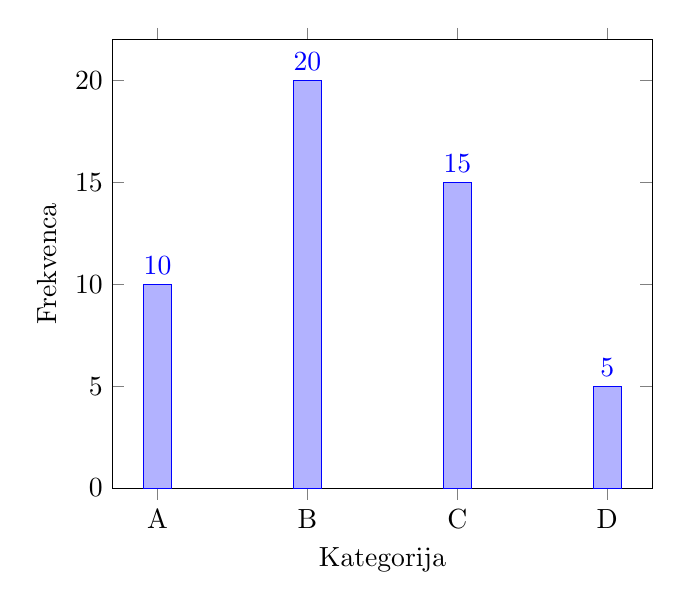
\begin{tikzpicture}
    \begin{axis}[
        ybar,
        symbolic x coords={A, B, C, D},
        xtick=data,
        ymin=0,
        ylabel={Frekvenca},
        xlabel={Kategorija},
        nodes near coords,
        ]
    \addplot coordinates {(A, 10) (B, 20) (C, 15) (D, 5)};
    \end{axis}
    \end{tikzpicture}
    \caption{Stolpčni grafikon frekvenc za nominalne spremenljivke.}
    \end{figure}

\section{Grafična predstavitev frelvenčnih porazdelitev za intervalne in razmernostne spremenljivke}

Histogram je vrsta stolpčnega grafikona, kjer stolpci predstavljajo frekvence podatkov v določenih intervalih. Histogram je uporaben za prikaz razpršenosti podatkov in za ugotavljanje oblik porazdelitev, kot so normalna, enakomerno porazdeljena ali pristranska porazdelitev.

\begin{figure}
    \centering
    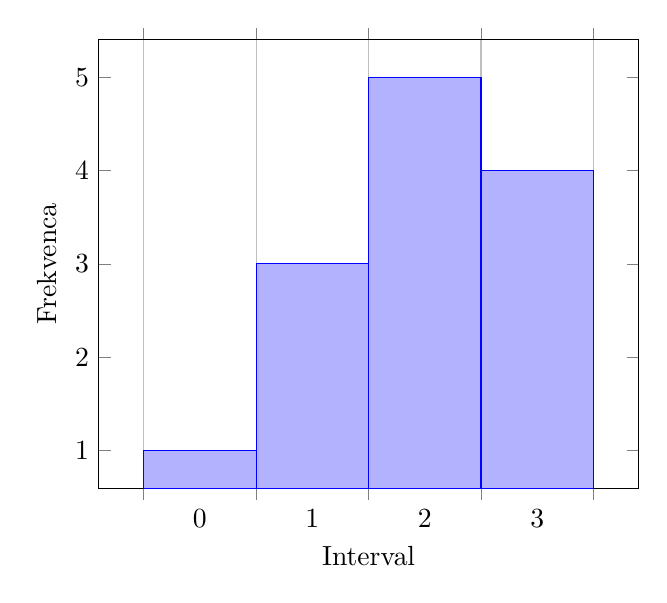
\begin{tikzpicture}
    \begin{axis}[
        ybar interval,
        ylabel={Frekvenca},
        xlabel={Interval},
        ]
    \addplot coordinates {(0, 1) (1, 3) (2, 5) (3, 4) (4, 2)};
    \end{axis}
    \end{tikzpicture}
    \caption{Histogram frekvenc za intervalne spremenljivke.}
\end{figure}

Poligon frekvenc je črtni grafikon, ki povezuje sosednje točke, ki predstavljajo frekvence intervalov. Uporablja se za prikaz porazdelitve podatkov in omogoča enostavno primerjavo z drugimi porazdelitvami.

\begin{figure}
    \centering
    \begin{tikzpicture}
    \begin{axis}[
        ylabel={Frekvenca},
        xlabel={Interval},
        ]
    \addplot coordinates {(0, 1) (1, 3) (2, 5) (3, 4) (4, 2)};
    \end{axis}
    \end{tikzpicture}
    \caption{Poligon frekvenc za intervalne spremenljivke.}
\end{figure}

Ogiva je črtni grafikon, ki prikazuje kumulativne frekvence. To pomeni, da vsaka točka na grafu predstavlja vsoto vseh prejšnjih frekvenc do določene vrednosti. Ogiva je uporabna za določanje percentilov in za primerjavo kumulativnih porazdelitev med različnimi skupinami podatkov.

\begin{figure}
    \centering
    \begin{tikzpicture}
    \begin{axis}[
        ylabel={Kumulativna frekvenca},
        xlabel={Interval},
        ]
    \addplot coordinates {(0, 1) (1, 4) (2, 9) (3, 13) (4, 15)};
    \end{axis}
    \end{tikzpicture}
    \caption{Ogiva za kumulativne frekvence.}
\end{figure}

\section{Normalna porazdelitev}

Normalna porazdelitev je ena izmed najpomembnejših verjetnostnih porazdelitev v statistiki in se pogosto uporablja pri modeliranju različnih naravnih in družbenih pojavov. Gostotna funkcija normalne porazdelitve je podana z naslednjo enačbo:

\[f_X(x) = \frac{1}{\sigma\sqrt{2\pi}} e^{-\frac{1}{2} \frac{(x-\mu)^2}{\sigma^2}},\]

kjer je $\mu$ povprečje (aritmetična sredina) in $\sigma$ standardni odklon. Graf normalne porazdelitve je zvonaste oblike in simetričen glede na povprečje $\mu$.

\begin{figure}
\centering
\begin{tikzpicture}
\begin{axis}[
    no markers, 
    domain=-4:4, 
    samples=100, 
    axis lines*=left, 
    xlabel=$x$, 
    ylabel=$f_X(x)$,
    height=6cm, 
    width=10cm, 
    xtick=\empty, 
    ytick=\empty,
    enlargelimits=false, 
    clip=false, 
    axis on top,
    grid = major
    ]
    \addplot[very thick,cyan!50!black] {1/(sqrt(2*pi))*exp(-x^2/2)};
\end{axis}
\end{tikzpicture}
\caption{Gostotna funkcija normalne porazdelitve.}
\end{figure}

\subsection{Asimetričnost (skewness)}

Asimetričnost meri, kako je porazdelitev nagnjena v levo ali desno. Normalna porazdelitev je popolnoma simetrična in ima koeficient asimetričnosti $k = 0$. Vendar pa v realnih podatkih pogosto srečamo porazdelitve, ki niso povsem simetrične:

\begin{itemize}
    \item Negativna asimetričnost (v levo, $k < 0$): Rep porazdelitve je daljši na levi strani.
    \item Pozitivna asimetričnost (v desno, $k > 0$): Rep porazdelitve je daljši na desni strani.
\end{itemize}

Če je $k$ med -1 in 1, se porazdelitev še vedno lahko šteje za normalno.

\begin{figure}
\centering
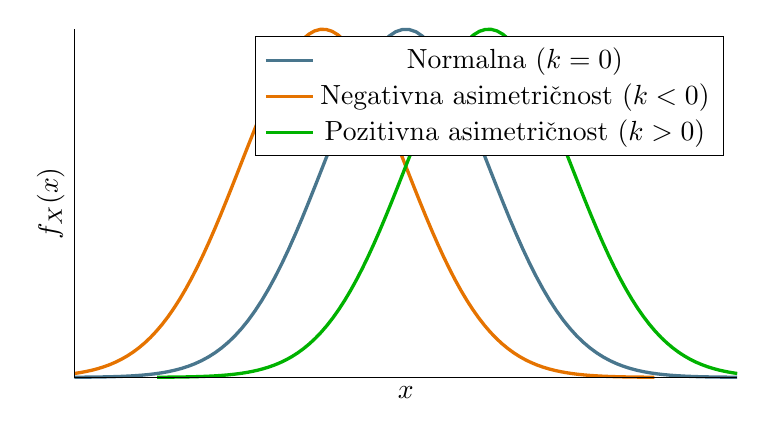
\begin{tikzpicture}
\begin{axis}[
    no markers, 
    domain=-4:4, 
    samples=100, 
    axis lines*=left, 
    xlabel=$x$, 
    ylabel=$f_X(x)$,
    height=6cm, 
    width=10cm, 
    xtick=\empty, 
    ytick=\empty,
    enlargelimits=false, 
    clip=false, 
    axis on top,
    grid = major
    ]
    \addplot[very thick,cyan!50!black] {1/(sqrt(2*pi))*exp(-x^2/2)};
    \addplot[very thick,orange!90!black, domain=-4:3] {1/(sqrt(2*pi))*exp(-((x+1)^2)/2)};
    \addplot[very thick,green!70!black, domain=-3:4] {1/(sqrt(2*pi))*exp(-((x-1)^2)/2)};
    \legend{Normalna ($k=0$), Negativna asimetričnost ($k<0$), Pozitivna asimetričnost ($k>0$)}
\end{axis}
\end{tikzpicture}
\caption{Grafi normalne porazdelitve s pozitivno in negativno asimetričnostjo.}
\end{figure}

\subsection{Sploščenost (kurtosis)}

Sploščenost meri, kako visoka in ostra je konica porazdelitve v primerjavi z normalno porazdelitvijo:

\begin{itemize}
    \item Leptokurtična ($k > 0$): Porazdelitev ima ožjo in višjo konico ter debelejše repe.
    \item Mezokurtična ($k = 0$): Porazdelitev je normalno zvonaste oblike.
    \item Platokurtična ($k < 0$): Porazdelitev ima ploščato konico in tanjše repe.
\end{itemize}

Če je $k$ med -1 in 1, se porazdelitev še vedno lahko šteje za normalno.

\begin{figure}
\centering
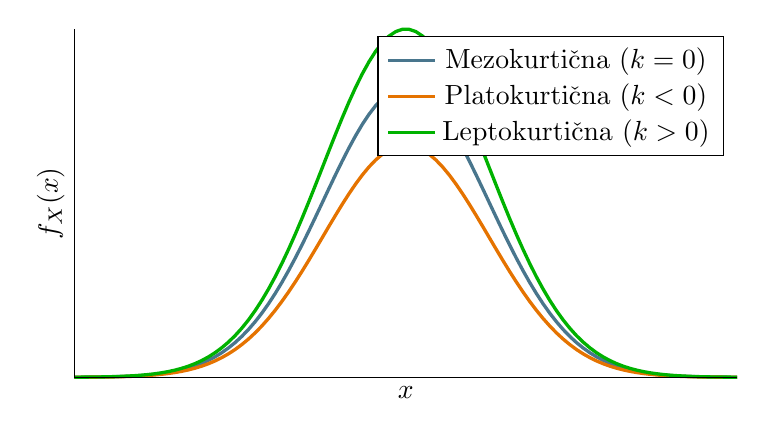
\begin{tikzpicture}
\begin{axis}[
    no markers, 
    domain=-4:4, 
    samples=100, 
    axis lines*=left, 
    xlabel=$x$, 
    ylabel=$f_X(x)$,
    height=6cm, 
    width=10cm, 
    xtick=\empty, 
    ytick=\empty,
    enlargelimits=false, 
    clip=false, 
    axis on top,
    grid = major
    ]
    \addplot[very thick,cyan!50!black] {1/(sqrt(2*pi))*exp(-x^2/2)};
    \addplot[very thick,orange!90!black] {0.8/(sqrt(2*pi))*exp(-x^2/2)};
    \addplot[very thick,green!70!black] {1.2/(sqrt(2*pi))*exp(-x^2/2)};
    \legend{Mezokurtična ($k=0$), Platokurtična ($k<0$), Leptokurtična ($k>0$)}
\end{axis}
\end{tikzpicture}
\caption{Grafi normalne porazdelitve s pozitivno in negativno sploščenostjo.}
\end{figure}

\section{Rangiranje}

Rangiranje vključuje razvrščanje podatkovnih točk v naraščajočem ali padajočem vrstnem redu. Rang določene vrednosti v podatkovnem naboru je njeno mesto v tem vrstnem redu. Rangiranje je uporabno za prepoznavanje relativnega položaja podatkovne točke znotraj nabora podatkov.

\textbf{Primer:}
\begin{itemize}
    \item Podatkovni niz: $45, 32, 67, 23, 89, 56$
    \item Urejeni podatkovni niz: $23, 32, 45, 56, 67, 89$
    \item Rangiranje: 
    \begin{itemize}
        \item 23 ima rang 1
        \item 32 ima rang 2
        \item 45 ima rang 3
        \item 56 ima rang 4
        \item 67 ima rang 5
        \item 89 ima rang 6
    \end{itemize}
\end{itemize}

\subsection{Kvantili}

Kvantili so vrednosti, ki delijo urejen niz podatkov na enake dele. Najpogosteje uporabljeni kvantili so kvartili, decili in percentili.

\textbf{Kvartili:}
Kvartili delijo podatkovni niz na štiri enake dele:
\begin{itemize}
    \item Prvi kvartil ($Q_1$): 25. percentil
    \item Drugi kvartil ($Q_2$): 50. percentil (median)
    \item Tretji kvartil ($Q_3$): 75. percentil
\end{itemize}

\textbf{Decili:}
Decili delijo podatkovni niz na deset enakih delov:
\begin{itemize}
    \item Prvi decil ($D_1$): 10. percentil
    \item Drugi decil ($D_2$): 20. percentil
    \item Tretji decil ($D_3$): 30. percentil
    \item itd.
\end{itemize}

\textbf{Percentili:}
Percentili delijo podatkovni niz na sto enakih delov:
\begin{itemize}
    \item 10. percentil: vrednost pod katero leži 10\% podatkov
    \item 50. percentil: vrednost pod katero leži 50\% podatkov (median)
    \item 90. percentil: vrednost pod katero leži 90\% podatkov
\end{itemize}

\textbf{Primer:}
Podatkovni niz: $15, 20, 35, 40, 50$
\begin{itemize}
    \item $Q_1$ (25. percentil): $20 + 0.25 \times (35 - 20) = 23.75$
    \item $Q_2$ (50. percentil): Median = $35$
    \item $Q_3$ (75. percentil): $35 + 0.75 \times (50 - 35) = 46.25$
\end{itemize}

\begin{figure}
\centering
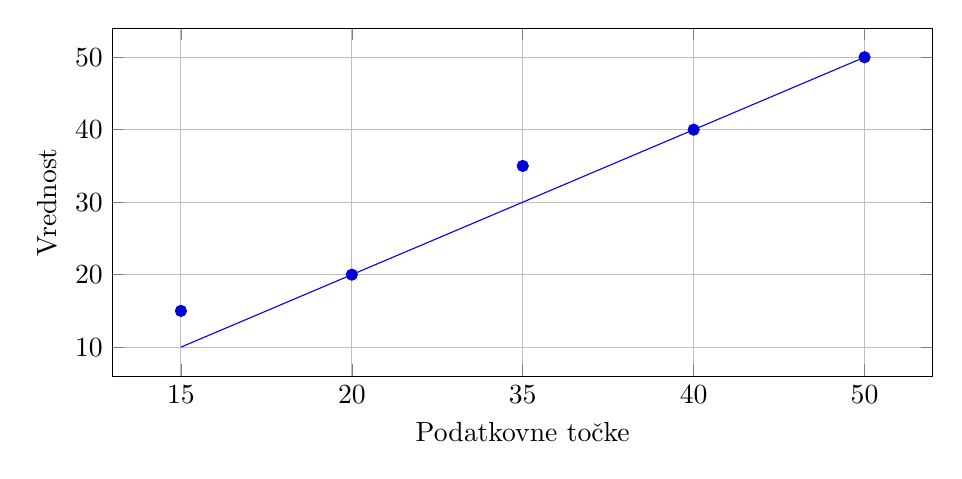
\begin{tikzpicture}
\begin{axis}[
    height=6cm,
    width=12cm,
    xtick={1, 2, 3, 4, 5},
    xticklabels={15, 20, 35, 40, 50},
    xlabel={Podatkovne točke},
    ylabel={Vrednost},
    ytick={0, 10, 20, 30, 40, 50, 60},
    grid=major
]
\addplot+[only marks,mark=*] coordinates {(1, 15) (2, 20) (3, 35) (4, 40) (5, 50)};
\addplot[domain=1:5, samples=5, color=blue] {x * 10};
\end{axis}
\end{tikzpicture}
\caption{Prikaz podatkovnega niza in kvantilov.}
\end{figure}

\section{Mere centralne tendence}
\begin{itemize}
    \item \textbf{Modus} - vrednost, ki se najpogosteje pojavi v nizu vrednosti podatkov
    \item \textbf{Mediana} - vrednost, ki ločuje zgornjo polovico obsega razpona vrednosti od spodnje polovice
    \item \textbf{Aritmetična sredina} - povprečje niza vrednosti
    \item Druge mere (geometrijska, harmonična sredina, ...)
\end{itemize}
Primerjava med modusom, mediano in aritmetično za unimodalne asimetrične - slika

\section{Mere variabilnosti (disperzije)}
V kolikšni meri se vrednosti razlikujejo med seboj ter razlikujejo in odstopajo od povprečja. Delimo jih na:
\begin{itemize}
    \item Absolutne mere (razpon, interkvartilni rang, absolutna deviacija aritmetične sredine/mediane, varianca in standardni odklon) 
    \item Relativne mere (absolutne mere deljene s pripadajočo mero centralne tendence) se izračunajo samo za razmernostne spremenljivke; uporabljamo jih, ko želimo primerjati:
    \begin{itemize}
        \item Dve porazdelitvi z zelo različno vrednostjo za nek mero centralne tendence;
        \item Dve spremenljivki z različnima merskima enotama.
    \end{itemize}
\end{itemize}

\subsection*{Razpon}

Absolutni razpon \[R_{abs}=x_{max}-x_{min}\]

Relativni razpon \[R_{rel}=\frac{2\left(x_{max}-x_{min}\right)}{x_{max}+x_{min}}\]

\subsection*{Interkvartilni rang}

\[IQR =\frac{Q_3 -Q_1}{2}\]

\subsection*{Absolutna deviacija mediane/aritmetične sredine}

\[AD_{Me,\mu}=\frac{1}{N}\sum_{i=1}^{N}|x_i - Me,\mu|\]

\subsection*{Varianca in standardni odklon}

\[\sigma^2 = \frac{1}{N} \sum_{i=1}^{N} (x_i - \mu)^2\]

\[\sigma = \sqrt{\sigma^2}\]

\subsection*{Variabilnost normalne porazdelitve}

Slika naslednjega

\begin{itemize}
    \item 68,3\% enot je znotraj enega standardnega odklona od povprečja \([\mu - \sigma, \mu + \sigma]\)
    \item 95,4\% enot je znotraj dveh standardnih odklonov od povprečja \([\mu - 2\sigma, \mu + 2\sigma]\)
    \item 99,7\% enot je znotraj treh standardnih odklonov od povprečja \([\mu - 3\sigma, \mu + 3\sigma]\)
\end{itemize}

\subsection*{Standardizacija}

\[z_i = \frac{x_i - \mu_X}{\sigma_X}\]

Rezultat je standardizirana spremenljivka $Z$, kjer standardizirane vrednosti $z_i$ predstavljajo relativna odstopanja od aritmetične sredine. Standardizacija nam omogoča primerjavo vrednosti različnih spremenljivk, ki praviloma niso primerljive.

Primer primerjave teže in višine dojenčkov, kjer standardiziramo glede na spol.

\begin{table}[h!]
    \centering
    \begin{tabular}{cccccc}
    \toprule
    Dojenček & Spol & Teža (kg) & $\mu_X$ (kg) & $\sigma_X$ (kg) & $z_i$ \\
    \midrule
    1 & Moški & 3.5 & 3.4 & 0.5 & $z_1 = \frac{3.5 - 3.4}{0.5} = 0.2$ \\
    2 & Ženski & 3.0 & 3.2 & 0.4 & $z_2 = \frac{3.0 - 3.2}{0.4} = -0.5$ \\
    3 & Moški & 4.0 & 3.4 & 0.5 & $z_3 = \frac{4.0 - 3.4}{0.5} = 1.2$ \\
    4 & Ženski & 2.8 & 3.2 & 0.4 & $z_4 = \frac{2.8 - 3.2}{0.4} = -1.0$ \\
    \bottomrule
    \end{tabular}
    \caption{Standardizacija teže dojenčkov glede na spol.}
\end{table}

\begin{Vaje}{1}
    Učence smo testirali v znanju matematike in dosegli so naslednje rezultate:
\[
\begin{array}{cccccccccccccc}
20 & 17 & 25 & 20 & 12 & 25 & 18 & 16 & 25 \\
17 & 21 & 22 & 22 & 16 & 17 & 22 & 20 & 19 & 16 \\
24 & 20 & 15 & 14 & 23 & 15 & 19 & 21 & 26 \\
18 & 29 & 30 & 20 & 16 & 12 & 24 & 30 & 27 & 25 \\
15 & 25 & 24 & 23 & 26 & 21 \\
\end{array}
\]

\begin{enumerate}
\item Poišči rezultat z rangom 8 (od najslabšega).
\item Koliko \% učencev je doseglo več kot 22 točk?
\item Kateri rezultat (ali rezultati) se najpogosteje pojavlja?
\item Rezultate testiranja razvrsti v frekvenčno porazdelitev.
\item Podatke prikaži grafično.
\end{enumerate}
\end{Vaje}

\begin{Vaje}{2} 
        Skupino desetih učencev smo testirali s psihodiagnostičnim testom in dobili naslednje rezultate:
        \[
        \begin{array}{cccccccccc}
        17 & 26 & 22 & 15 & 18 & 27 & 16 & 20 & 18 & 24 \\
        \end{array}
        \]
        
        \begin{enumerate}
            \item Izračunaj kvartile.
            \item Določi kvantilni rang vrednosti $x = 22.50$.
            \item Določi kvantilni rang rezultata $x = 22.00$.
        \end{enumerate}
\end{Vaje}

\begin{Vaje}{3}
    Na eni izmed avtošol smo se pozanimali, Koliko ur vožnje so kandidati potrebovali, preden so uspešno opravili vozniški izpit. Izračunaj aritmetično sredino, varianco in standardni odklon.
\end{Vaje}